\chapter{Simulation d'une inversion de stratification associée au transfert de masse}

Pour conclure l'étude, on cherche à modéliser le détachement de gouttelettes induites par transfert de masse. Le détachement est un cas important d'étude puisque c'est un phénomène déterminant pour l'étude de la stratification du bain de corium (\textit{cf.} Chapitre \ref{chap:1}). L'analyse du régime linéaire d'une instabilité de Rayleigh-Taylor dans TrioCFD a été effectuée dans \cite{rasolofomanana_modelisation_nodate} avec des résultats tout à fait satisfaisants. Ainsi, l'objectif de cette section est simplement d'observer un détachement de gouttelettes dans un système ternaire et une relocalisation en fond de domaine.
\section{Conditions initiales}
Le paysage choisi est la même que celui utilisé au chapitre précédent en notant les phases $\alpha$ et $\beta$, il est représenté en Figure \ref{fig:landchap5}, une fois de plus ce paysage nous conserve de tout problème lié au profil d'interface. Un schéma représentatif des conditions initiales est présenté en Figure \ref{fig:schema_RT}, initialement la phase $\alpha$ est plus légère que la phase $\beta$, puis sous l'effet de la diffusion de l'élément léger de la phase $\alpha$ vers la phase $\beta$, la phase $\alpha$ s'alourdit jusqu'au détachement de gouttelettes.	

\begin{figure}[H]
	\centering
\begin{subfigure}[ht!]{0.45\textwidth}
		\centering
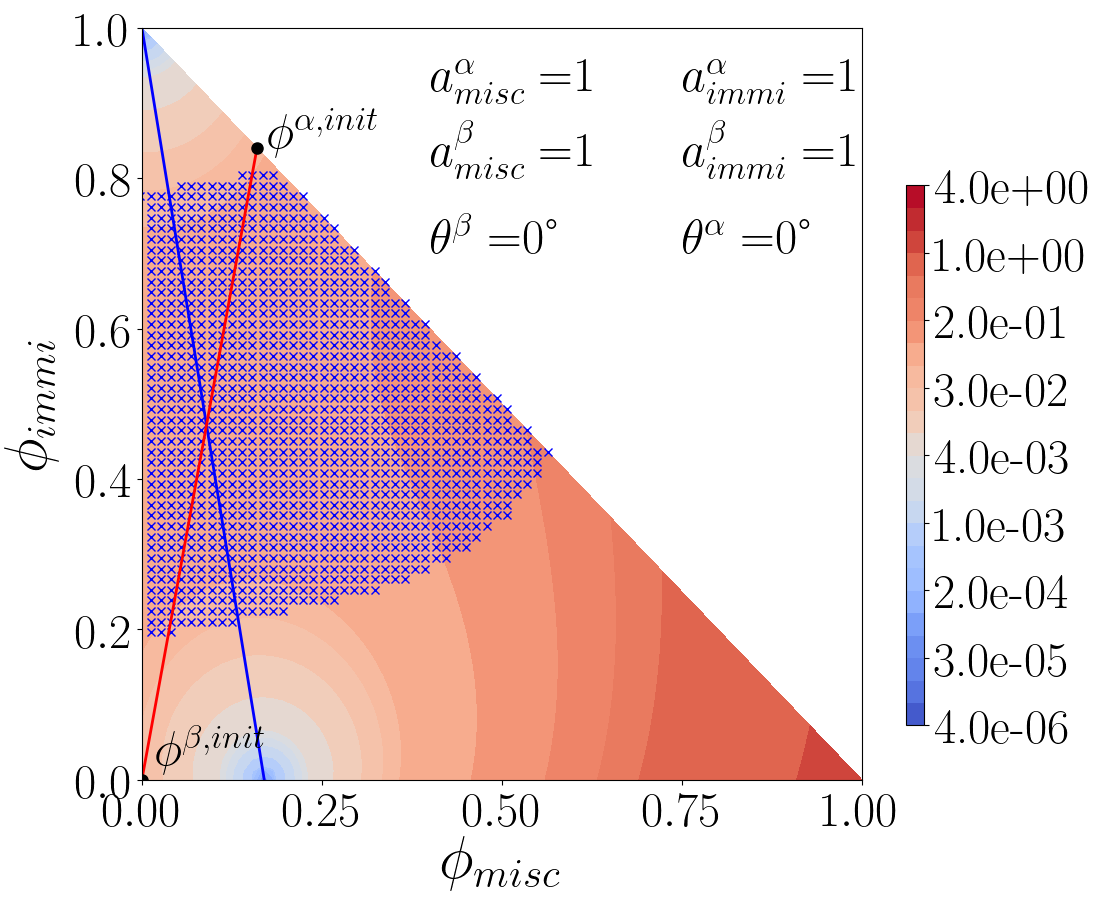
\includegraphics[width=1\textwidth]{figure/landscape_chap5.png}
\caption{Paysage thermodynamique}
\label{fig:landchap5}
\end{subfigure}
\begin{subfigure}[ht!]{0.45\textwidth}
	\centering
\begin{circuitikz}[scale=0.4]
	%		\oeil[shift={(3.5,5.2)},rotate=60,fill=white];
	%		\draw [-triangle 60] (4,6) -- (6,9);
	\begin{scope}[xshift=3cm]
		\draw [scale=1,thick] (0,0) -- (6,0) -- (6,12) -- (0,12) -- cycle;
		\draw [scale=1,thick] (0,9) -- (6,9) ;
		%\draw [scale=1,thick,dashed] (3,8) -- (3,10) ;
		\draw [scale=1,thick,dashed] (3,9) circle (0.8cm) node {};
		\draw [-triangle 60] (4,6) -- (3,9);
		\node (A) at (4,5) {perturb.};
		\node (A) at (3,1.7) {phase $\beta$};
		\node (B) at (3,11) {phase $\alpha$};
	\end{scope}
\end{circuitikz}
\caption{Schéma représentatif des conditions initiales}
\label{fig:schema_RT}
\end{subfigure}
\caption{Schéma représentatif des conditions initiales et paysage thermodynamique}
\label{fig:schema_RTetlandscape}
\end{figure}
Les simulations sont réalisées sur un système non-physique, ainsi, tout comme le paysage, la tension de surface et la viscosité sont choisies arbitrairement, la viscosité est cohérente avec le cas du corium, cependant la tension de surface est cinquante fois plus faible que l'ordre de grandeur de référence du corium. Les dimensions du système sont également fortement réduite par rapport à une cuve. Cependant les dimensions se rapprochent des essais mettant en jeu du corium prototypique en creuset froid MASCA-MA avec un creuset de 7cm de diamètre pour 2kg de corium, au cours desquels les inversions sont très rapide (<30 minutes). Les paramètres de la simulation sont présentés en Tableau \ref{table:cas_ref_RT}.
\begin{table}[H]
	\centering  % not needed, since table is as wide as text block
	\begin{tabularx}{\textwidth}{@{}lYYYYYY@{}}
		\toprule
		&\multicolumn{6}{c}{\bfseries Géométrie et maillage}\\
		%\cmidrule(lr){2-3} \cmidrule(l){4-5} 
		& $L_x$ (m)
		& $L_y$ (m)
		& $dx, dy$ (m)
		& $N_x$
		& $N_y$
		& $y_0$  (m)\\
		\midrule
		Valeurs  & 3.10$^{-2}$ & 5.10$^{-2}$ & 2.10$^{-4}$ & 150 & 500 & 0,037 \\
		\bottomrule
	\end{tabularx}
\end{table} \vspace{-0.8cm}
\begin{table}[H]
	\begin{tabularx}{\textwidth}{@{}lYYYYYY@{}}
		\toprule
		&\multicolumn{5}{c}{\bfseries Paramètres physiques}\\
		%\cmidrule(lr){2-3} \cmidrule(l){4-5} 
		& $\rho^*$ (kg.m$^{-3}$)
		& $\eta$ (Pa.s)
		& $\beta_{misc}$ (-)
		& $\beta_{immi}$ (-)
		& $\epsilon$ (m)\\
		\midrule
		Valeurs & 999,5 & 10$^{-3}$& -0,42 & 0,05 & 8.10$^{-4}$ \\
		\bottomrule
	\end{tabularx}
\end{table}\vspace{-0.8cm}
\begin{table}[H]
	\begin{tabularx}{\textwidth}{@{}lYYYY@{}}
		\toprule
		&\multicolumn{3}{c}{\bfseries Paramètres "champ de phase"}\\
		%\cmidrule(lr){2-3} \cmidrule(l){4-5} 
		& $\lambda$ (-)
		& $\kappa$
		& $\mathcal{M}$ (m$^2$.s$^{-1}$) \\
		\midrule
		Valeurs  & 27 & 2,16.10$^{-6}$ $\delta_{ij}$ & 1.10$^{-8}$ $\delta_{ij}$ \\	
		\bottomrule
	\end{tabularx}
\end{table}\vspace{-0.8cm}
\begin{table}[H]
	\begin{tabularx}{\textwidth}{@{}lYYYYYYYY@{}}
		\toprule
		&\multicolumn{8}{c}{\bfseries Conditions initiales et d'équilibres}\\
		%\cmidrule(lr){2-3} \cmidrule(l){4-5} 
		& $\phi_{misc}^{drop}$ 
		& $\phi_{immi}^{drop}$ 
		& $\phi_{misc}^{cont}$ 
		& $\phi_{immi}^{cont}$
		& $\phi_{misc}^{drop,eq}$ 
		& $\phi_{immi}^{drop,eq}$ 
		& $\phi_{misc}^{cont,eq}$ 
		& $\phi_{immi}^{cont,eq}$ \\
		\midrule
		Commun  & 0,12 & 0,87 & 0 & 0 & 0 & 1 & 0,17 & 0\\
		\bottomrule
	\end{tabularx}
	\caption{Paramètres des simulations} \label{table:cas_ref_RT}
\end{table}
Les conditions initiales de concentration peuvent s'écrire sous la forme :
\begin{equation}
\phi_{i}(\mathbf{x},t=0) = \frac{\phi^{init,\beta}_i + \phi^{init,\alpha}_i  }{2} +  \frac{\phi^{init,\beta}_i - \phi^{init,\alpha}_i }{2}\tanh\left(\frac{y-y_0+\gamma_1\exp\left(-\gamma_2 \text{rnd}\left(\cfrac{L_x}{2}-abs(x)\right)\right)}{\epsilon}\right)
\end{equation}
avec $\gamma_1, \gamma_2$ deux constantes, rnd$(u)$ un nombre pseudo-aléatoire compris entre $0$ et $u$, $L_x$ la largeur du domaine et $y_0$ la position de l'interface.\\
L'introduction de cette perturbation permet d'éviter le développement d'une instabilité mono-mode, de plus, sous l'effet de la diffusion initiale, permet d'introduire une excitation plus réaliste de l'interface.
\section{Résultats}
Les résultats sont présentés en Figure \ref{fig:rt1}, \ref{fig:rt2} et \ref{fig:rt3}. On y retrouve bien un détachement de gouttelettes menant à une inversion totale et une relocalisation en fond de domaine. Cependant, il est également possible d'observer que les parois du domaine semblent perturber légèrement le système. La Figure \ref{fig:profrhort} permet d'observer la diffusion massique dès les premiers instants du calcul menant à ce détachement de gouttelette.
\begin{figure}[H]
	\centering
	\begin{subfigure}[ht!]{0.2\textwidth}
		\centering
		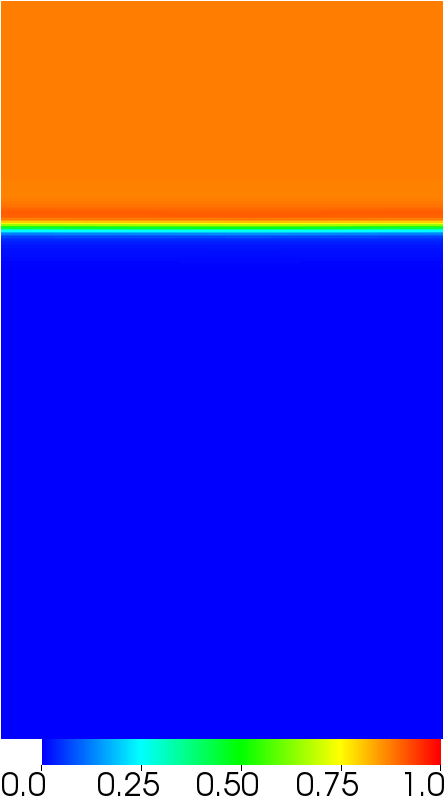
\includegraphics[width=1\textwidth]{figure/PT_RT/concent1/visit0000.png}
		\caption{$t=1s$}
	\end{subfigure}
	\begin{subfigure}[ht!]{0.2\textwidth}
		\centering
		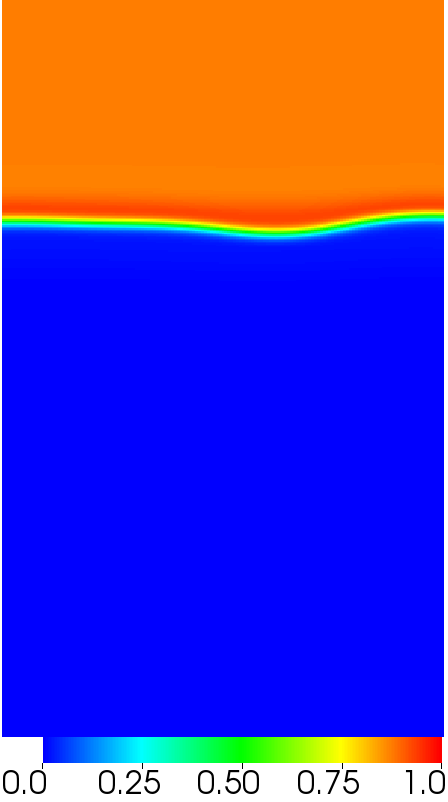
\includegraphics[width=1\textwidth]{figure/PT_RT/concent1/visit0001.png}
		\caption{$t=2s$}
	\end{subfigure}
	\begin{subfigure}[ht!]{0.2\textwidth}
		\centering
		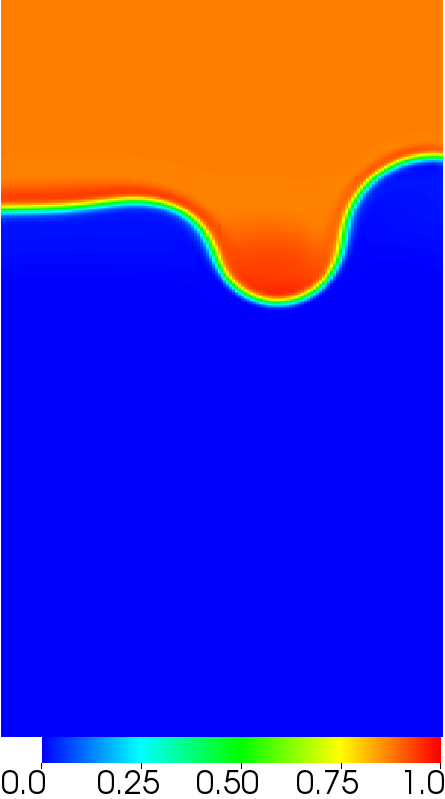
\includegraphics[width=1\textwidth]{figure/PT_RT/concent1/visit0002.png}
		\caption{$t=2,5s$}
	\end{subfigure}
	\begin{subfigure}[ht!]{0.2\textwidth}
		\centering
		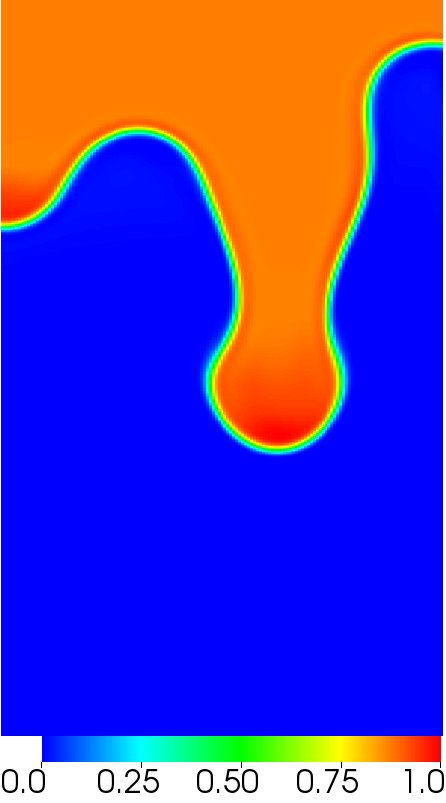
\includegraphics[width=1\textwidth]{figure/PT_RT/concent1/visit0003.png}
		\caption{$t=3s$}
	\end{subfigure}
\end{figure}\vspace{-0.8cm}
\begin{figure}[H]
	\centering
	\ContinuedFloat
	\begin{subfigure}[ht!]{0.2\textwidth}
		\centering
		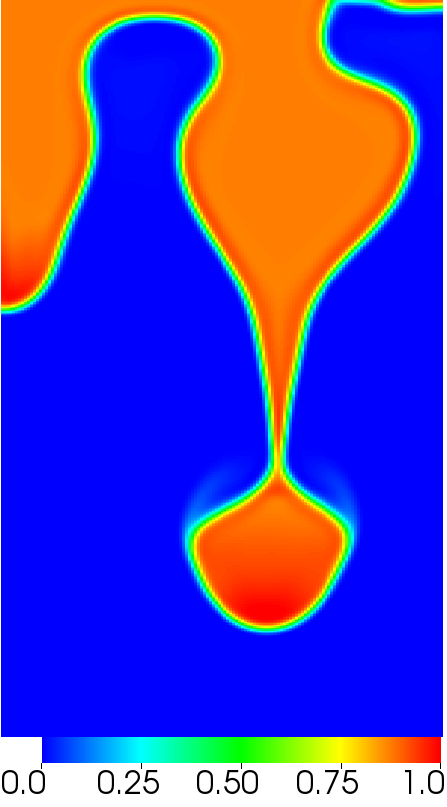
\includegraphics[width=1\textwidth]{figure/PT_RT/concent1/visit0004.png}
		\caption{$t=3,5s$}
	\end{subfigure}
	\begin{subfigure}[ht!]{0.2\textwidth}
		\centering
		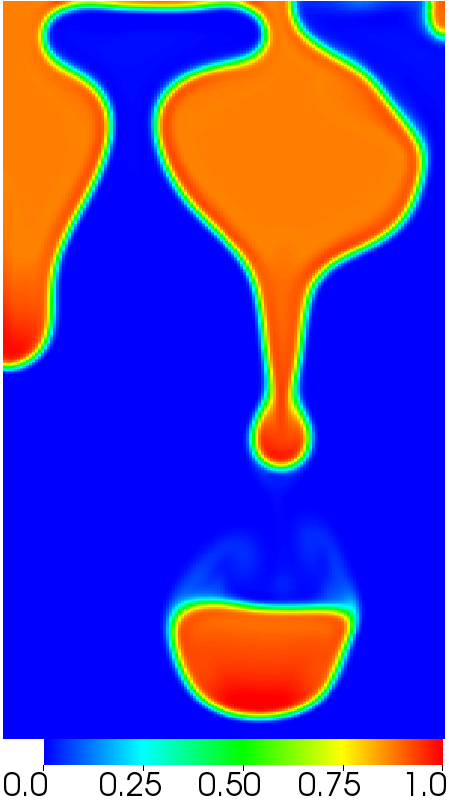
\includegraphics[width=1\textwidth]{figure/PT_RT/concent1/visit0005.png}
		\caption{$t=3,75s$}
	\end{subfigure}
	\begin{subfigure}[ht!]{0.2\textwidth}
		\centering
		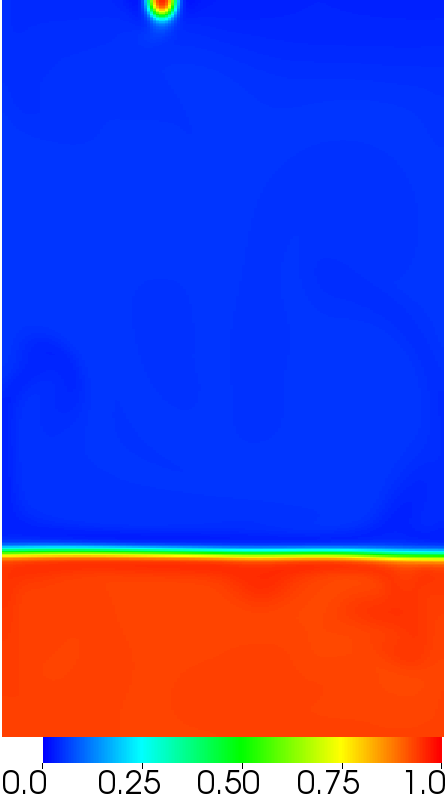
\includegraphics[width=1\textwidth]{figure/PT_RT/concent1/visit0006.png}
		\caption{$t=40s$}
	\end{subfigure}
	\caption{Champ de concentration de l'élément immiscible}
	\label{fig:rt1}
\end{figure}


\begin{figure}[H]
	\centering
	\begin{subfigure}[ht!]{0.2\textwidth}
		\centering
		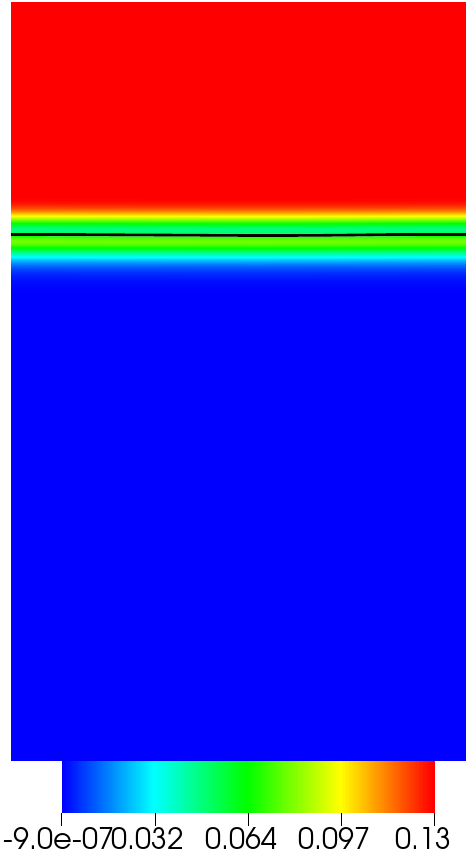
\includegraphics[width=1\textwidth]{figure/PT_RT/concent0/visit0007.png}
		\caption{$t=1s$}
	\end{subfigure}
	\begin{subfigure}[ht!]{0.2\textwidth}
		\centering
		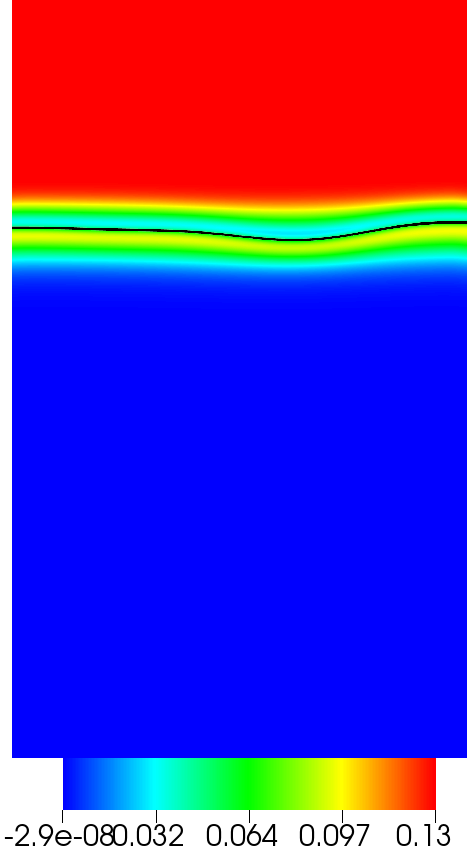
\includegraphics[width=1\textwidth]{figure/PT_RT/concent0/visit0008.png}
		\caption{$t=2s$}
	\end{subfigure}
	\begin{subfigure}[ht!]{0.2\textwidth}
		\centering
		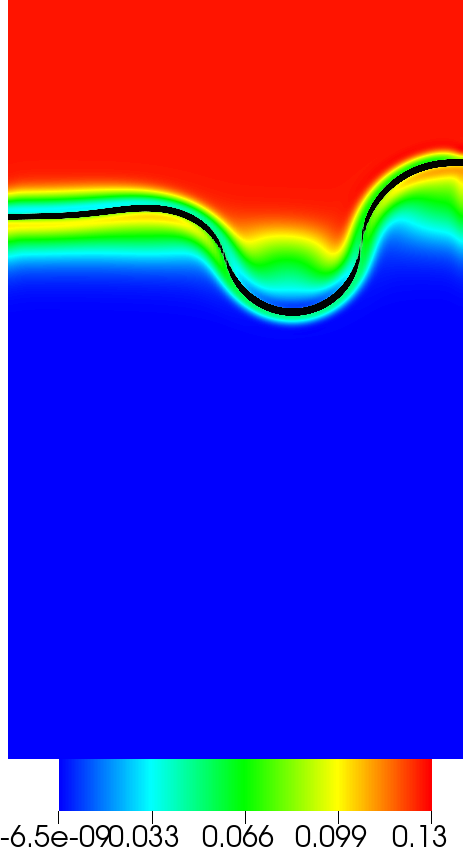
\includegraphics[width=1\textwidth]{figure/PT_RT/concent0/visit0009.png}
		\caption{$t=2,5s$}
	\end{subfigure}
	\begin{subfigure}[ht!]{0.2\textwidth}
		\centering
		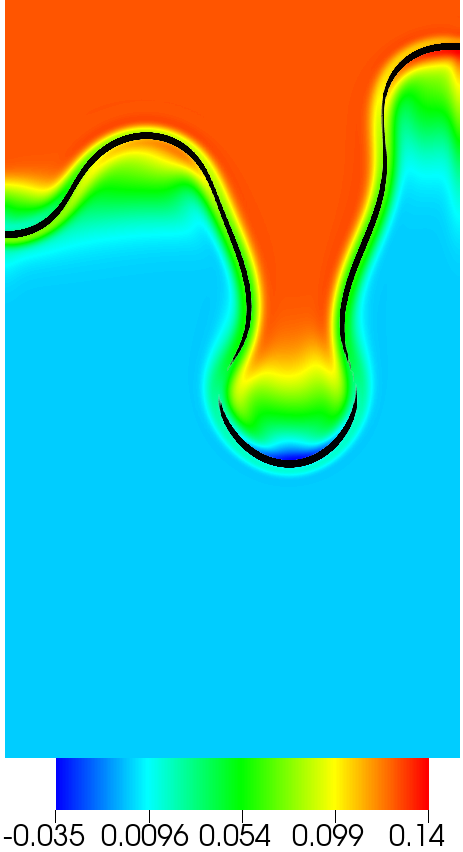
\includegraphics[width=1\textwidth]{figure/PT_RT/concent0/visit0010.png}
		\caption{$t=3s$}
	\end{subfigure}
\end{figure}\vspace{-0.8cm}
\begin{figure}[H]
	\centering
	\ContinuedFloat
	\begin{subfigure}[ht!]{0.2\textwidth}
		\centering
		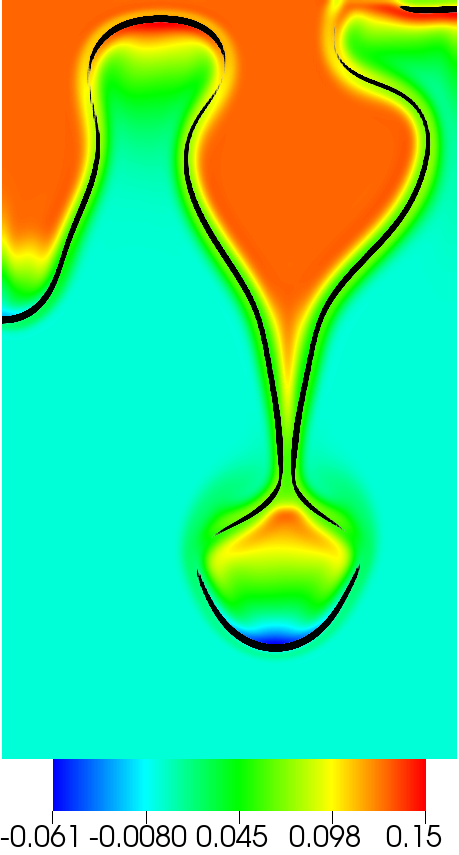
\includegraphics[width=1\textwidth]{figure/PT_RT/concent0/visit0011.png}
		\caption{$t=3,5s$}
	\end{subfigure}
	\begin{subfigure}[ht!]{0.2\textwidth}
		\centering
		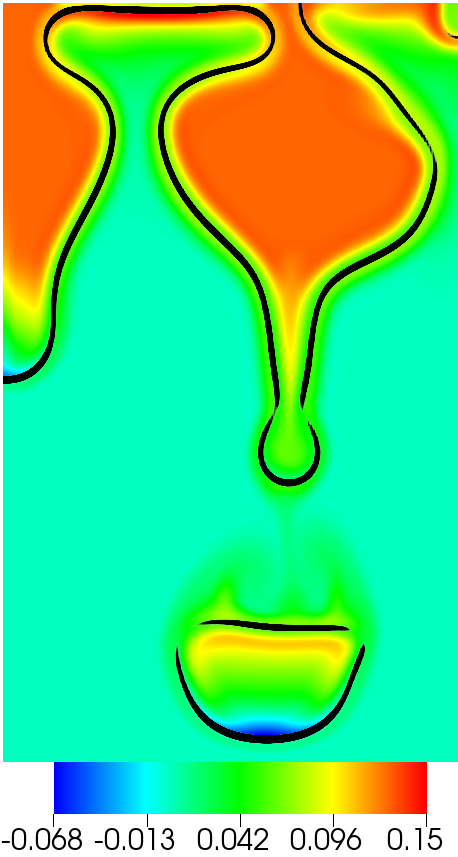
\includegraphics[width=1\textwidth]{figure/PT_RT/concent0/visit0012.png}
		\caption{$t=3,75s$}
	\end{subfigure}
	\begin{subfigure}[ht!]{0.2\textwidth}
		\centering
		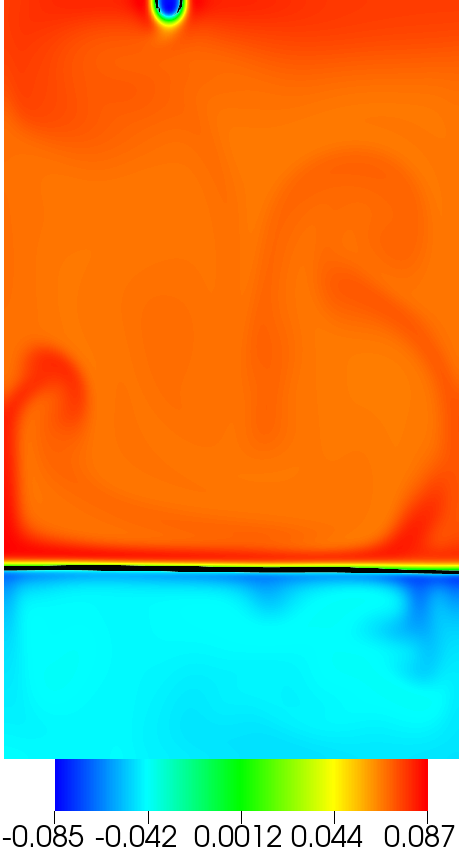
\includegraphics[width=1\textwidth]{figure/PT_RT/concent0/visit0013.png}
		\caption{$t=40s$}
	\end{subfigure}
	\caption{Champ de concentration de l'élément miscible}
	\label{fig:rt2}
\end{figure}


\begin{figure}[H]
	\centering
	\begin{subfigure}[ht!]{0.2\textwidth}
		\centering
		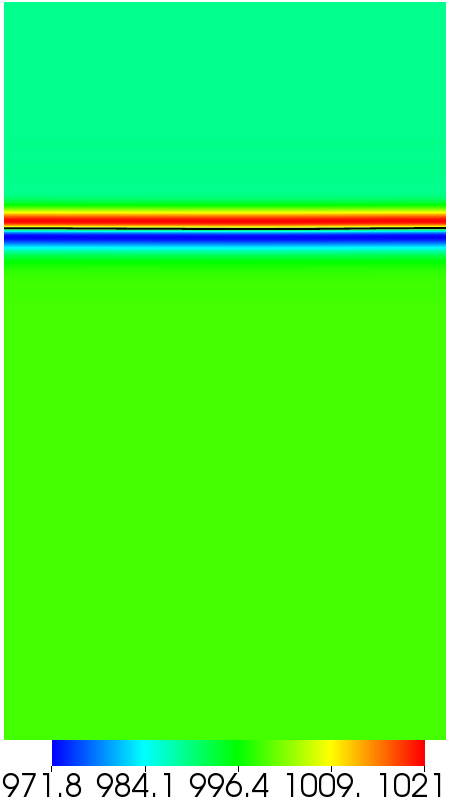
\includegraphics[width=1\textwidth]{figure/PT_RT/masse_vol/visit0014.png}
		\caption{$t=1s$}
	\end{subfigure}
	\begin{subfigure}[ht!]{0.2\textwidth}
		\centering
		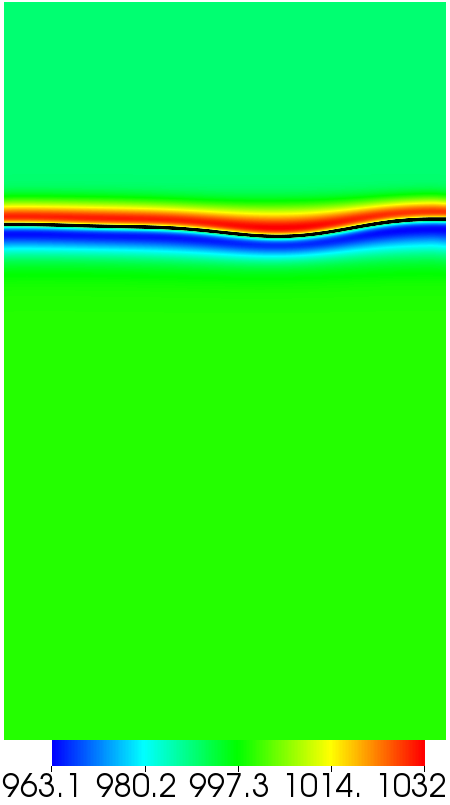
\includegraphics[width=1\textwidth]{figure/PT_RT/masse_vol/visit0015.png}
		\caption{$t=2s$}
	\end{subfigure}
	\begin{subfigure}[ht!]{0.2\textwidth}
		\centering
		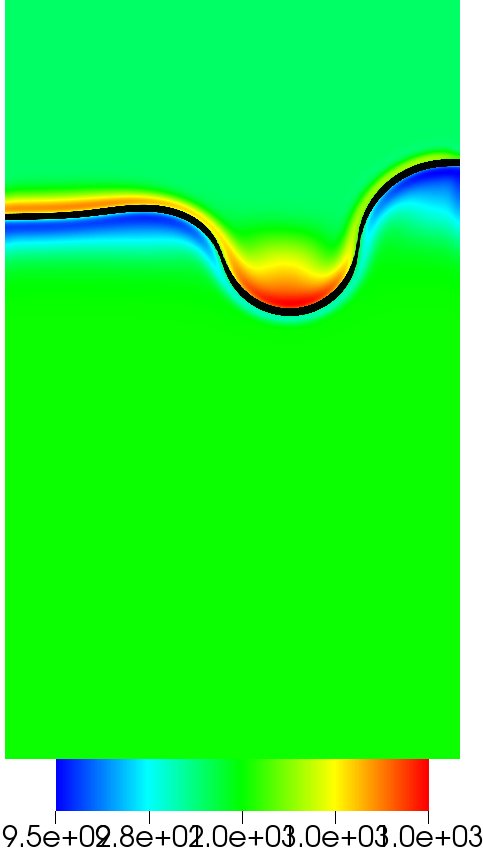
\includegraphics[width=1\textwidth]{figure/PT_RT/masse_vol/visit0020.png}
		\caption{$t=2,5s$}
	\end{subfigure}
	\begin{subfigure}[ht!]{0.2\textwidth}
		\centering
		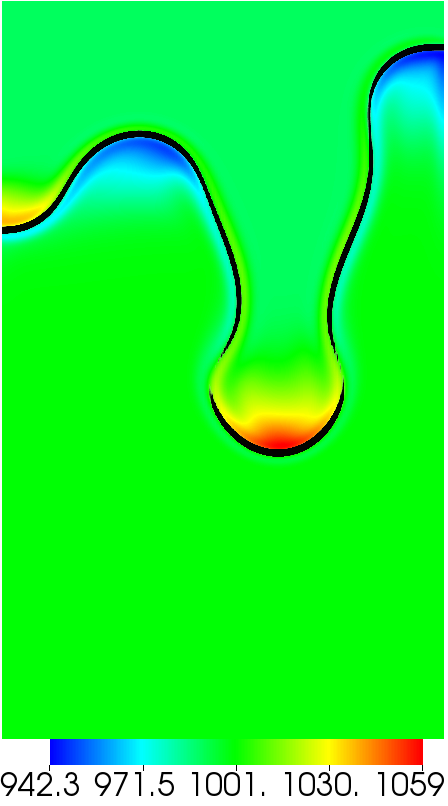
\includegraphics[width=1\textwidth]{figure/PT_RT/masse_vol/visit0016.png}
		\caption{$t=3s$}
	\end{subfigure}
\end{figure}\vspace{-0.8cm}
\begin{figure}[H]
	\centering
	\ContinuedFloat
	\begin{subfigure}[ht!]{0.2\textwidth}
		\centering
		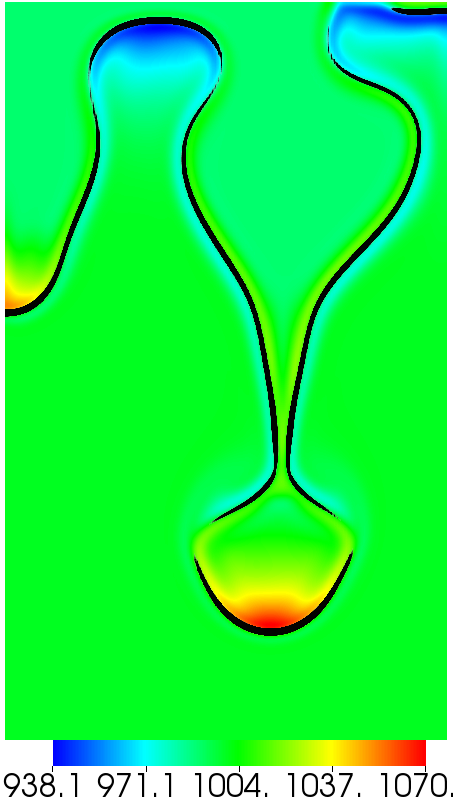
\includegraphics[width=1\textwidth]{figure/PT_RT/masse_vol/visit0017.png}
		\caption{$t=3,5s$}
	\end{subfigure}
	\begin{subfigure}[ht!]{0.2\textwidth}
		\centering
		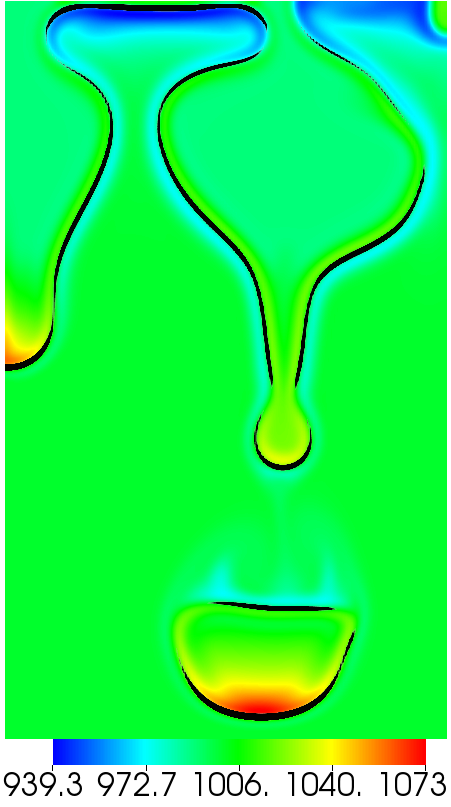
\includegraphics[width=1\textwidth]{figure/PT_RT/masse_vol/visit0018.png}
		\caption{$t=3,75s$}
	\end{subfigure}
	\begin{subfigure}[ht!]{0.2\textwidth}
		\centering
		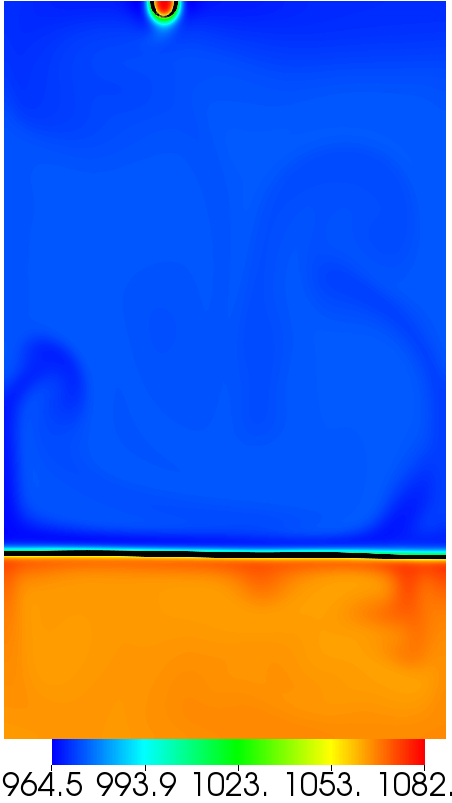
\includegraphics[width=1\textwidth]{figure/PT_RT/masse_vol/visit0019.png}
		\caption{$t=40s$}
	\end{subfigure}
	\caption{Champ de masse volumique}
	\label{fig:rt3}
\end{figure}
\begin{minipage}{0.2\textwidth}\hspace{-1cm}
	\begin{circuitikz}[scale=0.4]
		\oeil[shift={(3.5,5.2)},rotate=60,fill=white];
		\draw [-triangle 60] (4,6) -- (6,9);
		\begin{scope}[xshift=3cm]
			\draw [scale=1,thick] (0,0) -- (6,0) -- (6,12) -- (0,12) -- cycle;
			\draw [scale=1,thick] (0,9) -- (6,9) ;
			\draw [scale=1,thick,dashed] (3,8) -- (3,10) ;
			%\draw [scale=1,thick,dotted] (3,9) circle (0.8cm) node {};
			\node (A) at (3,1.7) {fluide $\beta$};
			\node (B) at (3,11) {fluide $\alpha$};
		\end{scope}
	\end{circuitikz}
\end{minipage} \hspace{-2cm}
\begin{minipage}{0.8\textwidth}
	\begin{figure}[H]
		\centering
		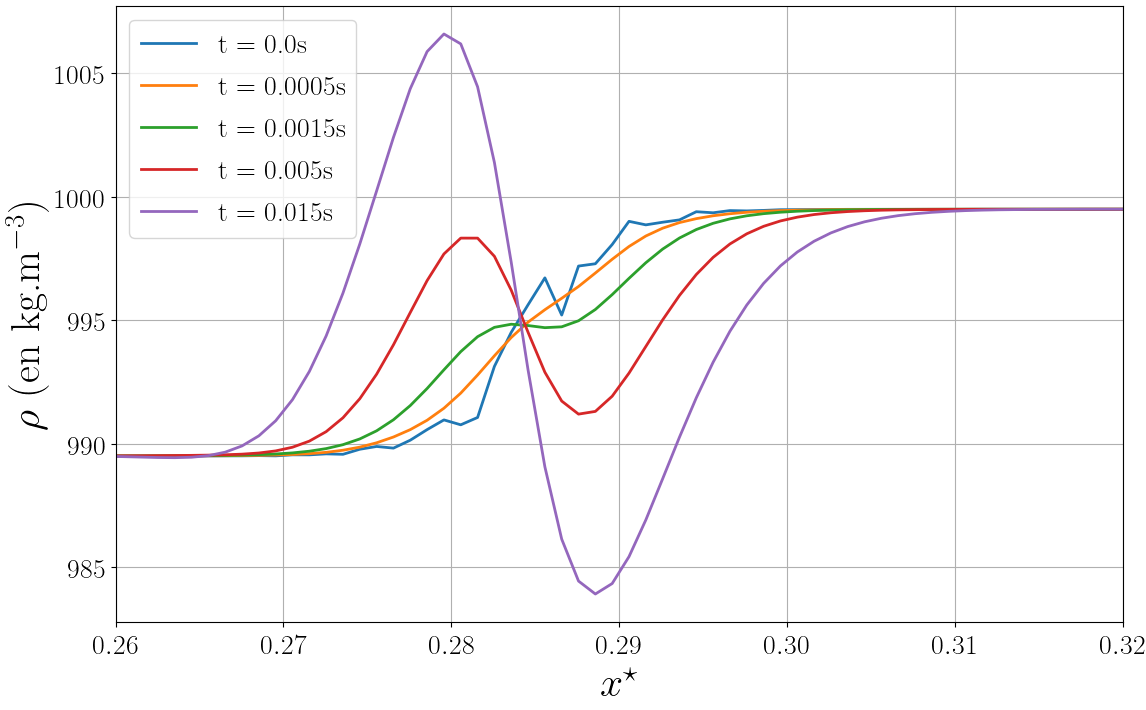
\includegraphics[width=0.8\linewidth]{figure/prof_rho_RT}
		\caption{Profil de masse volumique lors des premiers instants}
		\label{fig:profrhort}
	\end{figure}
\end{minipage} \\

Finalement, dans ce dernier chapitre, nous avons pu observer la capacité du code à reproduire des comportements hydrodynamiques d'intérêt pour l'étude de la stratification du corium. 


\chapter*{Conclusion}

Ce stage a finalement permis de participer à la validation d'un code CFD implémenté dans TrioCFD dans le cadre de la thèse de M.A Rasolofomanana \cite{rasolofomanana_modelisation_nodate}. Une expérience de la littérature couplant transfert de masse et hydrodynamique a pu être reproduite qualitativement et l'influence d'un nombre important de paramètres a pu être étudiée. Ce stage a également permis de retravailler sur le paramétrage du modèle champ de phase multicomposant en mettant en lumière certaines incompatibilités entre paysages et paramètres. \\
Une validation des régimes de déformation de goutte a également pu être menée permettant de participer à la validation dans un cas simplifié (sans transfert de masse). \\
Finalement, un comportement physique d'intérêt pour le laboratoire et la thématique accident grave a pu être simulé qualitativement permettant d'imaginer la réalisation de simulation quantitative dans le futur.

Les perspectives liées a ce travail sont multiples, sur le moyen terme une meilleure compréhension du potentiel thermodynamique analytique. La suite logique de ce travail serait également de proposer une formulation anisotherme pour permettre sur le long terme des simulations complètes couplant la thermohydraulique et la thermochimie d'un bain de corium.

Sur le plan personnel, ce stage m'a permis d'aborder des modèles complexes encore en développement et a conforté mon envie de réaliser une thèse orientée modélisation et calcul scientifique.



